\setchapterpreamble[u]{\margintoc}
\chapter{Контекстно-свободные языки и грамматики}
\label{CFG}
\tikzsetfigurename{CFG_}

Контекстно-свободные языки, являясь строгим расширением регулярных, находят своё применение в различных задачах анализа программного кода, биоинформатики~\sidecite{!!!}, и других задачах анализа данных.

\section{Основные определения}

\begin{definition}[Контекстно-свободная грамматика]
    \emph{Контекстно-свободная грамматика}~--- это четвёрка вида $\langle \Sigma, N, P, S \rangle$, где
    \begin{itemize}
        \item $\Sigma$~--- это терминальный алфавит;
        \item $N$~--- это нетерминальный алфавит;
        \item $P$~--- это множество правил (продукций), таких что каждая продукция имеет вид $N_i \to \alpha$, где $N_i \in N$ и $\alpha \in \{\Sigma \cup N\}^* \cup {\varepsilon}$;
        \item $S$~--- стартовый нетерминал.
              Отметим, что $\Sigma \cap N = \varnothing$.
    \end{itemize}
\end{definition}

\begin{example}
    \label{ex:binary_cfg}
    Грамматика, задающая язык целых чисел в двоичной записи без лидирующих нулей: $G = \langle \{0, 1, -\}, \{S, N, A\}, P, S \rangle$, где $P$ определено следующим образом:
    \begin{align*}
        S & \rightarrow 0 \mid N \mid - N              \\
        N & \rightarrow 1 A                            \\
        A & \rightarrow 0 A \mid 1 A  \mid \varepsilon
    \end{align*}
\end{example}

При спецификации грамматики часто опускают множество терминалов и нетерминалов, оставляя только множество правил.
При этом нетерминалы часто обозначаются прописными латинскими буквами, терминалы~--- строчными, а стартовый нетерминал обозначается буквой $S$.
Мы будем следовать этим обозначениям, если не указано иное.

\begin{definition}[Отношение непосредственной выводимости]
    \label{def derivability in CFG}
    \emph{Отношение непосредственной выводимости}. Мы говорим, что последовательность терминалов и нетерминалов $\gamma \beta \delta$ \emph{непосредственно выводится из} $\gamma \alpha \delta$ \emph{при помощи правила} $\alpha \rightarrow \beta$ ($\gamma \alpha \delta \derives[] \gamma \beta \delta$), если
    \begin{itemize}
        \item $\alpha \rightarrow \beta \in P$,
        \item $\gamma, \delta \in \{\Sigma \cup N\}^* \cup {\varepsilon}$.
    \end{itemize}
\end{definition}

\begin{definition}[Рефлексивно-транзитивное замыкание отношения]
    \emph{Рефлексивно-транзитивное замыкание отношения}~--- это наименьшее рефлексивное и транзитивное отношение, содержащее исходное.
\end{definition}

\begin{definition}[Отношение выводимости]
    \emph{Отношение выводимости} является рефлексивно-транзитивным замыканием отношения непосредственной выводимости; обозначается $\derives$.
    \begin{itemize}
        \item $\alpha \derives \beta$ означает $\exists \gamma_0, \dots, \gamma_k \in \{\Sigma \cup N\}^* \cup {\varepsilon}$:
              \[ \alpha \derives[] \gamma_0 \derives[] \gamma_1 \derives[] \dots \derives[] \gamma_{k-1} \derives[] \gamma_{k} \derives[] \beta;\]
        \item Транзитивность: $\forall \alpha, \beta, \gamma \in \{\Sigma \cup N\}^* \cup {\varepsilon}$: $\alpha \derives \beta$, $\beta \derives \gamma \derives[] \alpha \derives \gamma$;
        \item Рефлексивность: $\forall \alpha \in \{\Sigma \cup N\}^* \cup {\varepsilon}$: $\alpha \derives \alpha$;
        \item $\alpha \derives \beta$~--- $\alpha$ выводится из $\beta$;
        \item $\alpha \derives[k] \beta$~--- $\alpha$ выводится из $\beta$ за $k$ шагов;
        \item $\alpha \derives[+] \beta$~--- при выводе использовалось хотя бы одно правило грамматики.
    \end{itemize}
\end{definition}

\begin{example}
    Пример вывода цепочки $-1101$ в грамматике из примера~\ref{ex:binary_cfg}:
    \[
        S \derives[] - N \derives[] - 1 A \derives[] - 1 1 A \derives - 1 1 0 1 A \derives[] - 1 1 0 1
    \]
\end{example}

\begin{definition}[Вывод слова в грамматике]
    Слово $\omega \in \Sigma^*$ \emph{выводимо в грамматике} $\langle \Sigma, N, P, S \rangle$, если существует некоторый вывод этого слова из начального нетерминала $S \derives \omega$.

\end{definition}

\begin{definition}[Левосторонний вывод]
    \emph{Левосторонний вывод}. На каждом шаге вывода заменяется самый левый нетерминал.
\end{definition}

\begin{definition}[Правосторонний вывод]
    \emph{Правосторонний вывод}. На каждом шаге вывода заменяется самый правый нетерминал.
\end{definition}

\begin{example}
    Приведем пример левостороннего вывода цепочки $cbaa$ в грамматике:
    \begin{align*}
        S & \rightarrow A A \mid s          \\
        A & \rightarrow A A \mid B b \mid a \\
        B & \rightarrow c \mid d
    \end{align*}
    Жирным выделен нетерминал, заменяемый на каждом шагу вывода.
    \[ \mathbf{S} \derives[] \mathbf{A} A \derives[] \mathbf{B} b A \derives[] c b \mathbf{A} \derives[] c b \mathbf{A} A \derives[] c b a \mathbf{A} \derives[] c b a a \]
\end{example}

Аналогично левостороннему можно определить правосторонний вывод.

\begin{definition}[Язык]
    \emph{Язык, задаваемый грамматикой}~--- множество строк, выводимых в грамматике $L(G) = \{ \omega \in \Sigma^* \mid S \derives \omega \}$.
\end{definition}

\begin{definition}[Эквивалентные грамматики]
    Грамматики $G_1$ и $G_2$ называются \emph{эквивалентными}, если они задают один и тот же язык: $L(G_1) = L(G_2)$
\end{definition}

\begin{example}  Пример эквивалентных грамматик для языка целых чисел в двоичной системе счисления.

    \begin{tabular}{p{0.4\textwidth} | p{0.5\textwidth}}
        \[
            \begin{aligned}
                \Sigma & = \{ 0, 1, - \}                            \\
                N      & = \{ S, N, A \}                            \\~\\
                S      & \rightarrow 0 \mid N \mid - N              \\
                N      & \rightarrow 1 A                            \\
                A      & \rightarrow 0 A \mid 1 A  \mid \varepsilon \\
            \end{aligned}
        \]
         &
        \[
            \begin{aligned}
                \Sigma & = \{ 0, 1, - \}                            \\
                N      & = \{ S, A \}                               \\~\\
                S      & \rightarrow 0 \mid 1 A  \mid - 1 A         \\
                A      & \rightarrow 0 A \mid 1 A  \mid \varepsilon \\
            \end{aligned}
        \]
    \end{tabular}

\end{example}


\begin{definition}[Неоднозначная грамматика]
    \emph{Неоднозначная грамматика}~--- грамматика, в которой существует 2 и более левосторонних (правосторонних) выводов для одного слова.
\end{definition}

\begin{example}
    Неоднозначная грамматика для правильных скобочных последовательностей:
    \[
        S \to (S) \mid S S \mid \varepsilon
    \]
    Два различных левосторонних вывода строки $()()()$:
    \begin{gather*}
        S \derives[] S S \derives [] (S) S \derives[] () S \derives[] () S S \derives[] () (S) S \derives[] () () S \derives[] () () (S) \derives[] () () ()\\
        S \derives[] S S \derives[] S S S \derives[] (S) S S \derives[] () S S \derives[] () (S) S \derives[] () () S \derives[] () () (S) \derives[] () () ()
    \end{gather*}
\end{example}

\begin{definition}[Однозначная грамматика]
    \emph{Однозначная грамматика}~--- грамматика, в которой существует не более одного левостороннего (правостороннего) вывода для каждого слова.
\end{definition}

\begin{example}
    Однозначная грамматика для правильных скобочных последовательностей
    \[
        S \to (S)S \mid \varepsilon
    \]
\end{example}

\begin{definition}[Существенно неоднозначный язык]
    \emph{Существенно неоднозначные языки}~--- языки, для которых невозможно построить однозначную грамматику.
\end{definition}

\begin{example}
    Пример существенно неоднозначного языка
    \[\{a^n b^n c^m \mid n, m \in \BbbZ\} \cup \{a^n b^m c^m \mid n,m \in \BbbZ\}\]
\end{example}

\section{Рекурсивные автоматы и сети}

Рекурсивный автомат (Recursive state machine, RSM)~\sidecite{10.1145/1075382.1075387} или сеть~--- это представление контекстно-свободных грамматик, обобщающее конечные автоматы.
В нашей работе мы будем придерживаться термина \emph{рекурсивный автомат}.
Классическое определение рекурсивного автомата выглядит следующим образом.

\begin{definition}
    \emph{Рекурсивный автомат}~--- это кортеж $\mathcal{R} = \langle \mathcal{N},\Sigma,B,B_S,Q,Q_S\rangle$ where
    \begin{itemize}
       \item $N$~--- множество нетерминальных символов, 
       \item $\Sigma$~--- множество терминальных символов, 
       \item $Q$~--- множество состояний рекурсивного автомата, 
       \item $Q_S$~--- множество стартовых состояний всех \emph{блоков}, 
       \item $B=\{B_{N_i} \mid N_i \in \mathcal{N}\}$~--- множество блоков, где каждый \\ $B_{N_i} = \langle Q_{N_i}, q_S, Q_F^{N_i}, \delta \rangle$~--- это детерминированный конечный автомат, называемый \emph{блоком}.
             Здесь:  
            \begin{itemize}
                \item $Q_{N_i} \subseteq Q$~--- множество состояний блока, 
                \item $q_S \in Q_{N_i} \cap Q_S$~--- стартовое состояние блока, 
                \item $Q_F^{N_i} \subseteq Q_{N_i}$~--- множество финальных состояний блока, 
                \item $\delta \subseteq Q_{N_i} \times  (\Sigma\cup Q_S) \times Q_{N_i}$~--- функция переходов блока.
            \end{itemize}
       \item $B_S \in B$~--- стартовый блок рекурсивного автомата.
    \end{itemize}
\end{definition}

Таким образом, рекурсивный автомат~--- это набор детерминированных конечных автоматов над алфавитом $\Sigma \cup Q_S$.
В некоторых случаях наб будет удобно рассматривать этот набор как одн конечный автомат.
Однако процесс работы рекурсивного автомата несколько отличается от работы конечного автомата, хотя и похож на него.
Основное отличие~--- необходимость использовать стек для обработки переходов, помеченных элементами из $Q_S$.

По аналогии с конечными автоматами, процесс работы рекурсивных автоматов достаточно естественно описывается в терминах переходов между \emph{конфигурациями}.

\begin{definition}
    \emph{Конфигурация} $C_{\mathcal{R}}$ рекурсивного автомата $\mathcal{R}=\langle \mathcal{N},\Sigma,B,B_S,Q,Q_S \rangle$ over the graph $D=\langle V,E,L \rangle$ is a tuple $(q,v,\mathcal{S})$ where 
    \begin{itemize}
        \item $q \in Q$ is a current state of RSM,
        \item $\mathcal{S}$ is the current stack, whose frames have one of two types: 
        \begin{itemize} 
            \item return addresses frame (elements of $Q$) to specify states to continue computation after the call is finished;
            \item parsing tree node to store fragments of a parsing tree,
        \end{itemize}
        \item $v \in V$ is the current vertex (current position in the input).
    \end{itemize}
\end{definition}

\begin{definition}\label{def:rsm_transition}
    A \emph{transition step} of the RSM specifies how to get new configurations of RSM, given the current configuration. $C_{\mathcal{R}} \vdash W$ denotes that $\mathcal{R}$ can go to each configuration in $W$ from the configuration $C_{\mathcal{R}}$.
    \begin{align*}
    (q,v,w_0::s::\mathcal{S})  \vdash & \{ (q',v',t::w_0::s::\mathcal{S}) \mid (q,t,q') \in \delta, (v,t,v') \in E\} \\
                       & \cup \{(s', v, q'::w_0::s::\mathcal{S}) \mid (q,s',q') \in \delta, s' \in Q_S \} \\
                       & \cup \{(s,v,\emph{Node}(N_i, w_0)::\mathcal{S}) \mid q \in Q_F^{N_i}\}
    \end{align*}
    where $w_0$ is a possibly empty sequence of terminals and nonterminal nodes. 
\end{definition}

To simplify the acceptance condition, we introduce the concept of an \textit{extended RSM}. 

\begin{definition}
    For the given RSM $\mathcal{R}=\langle \mathcal{N},\Sigma,B,B_S,Q,Q_S\rangle$,
    the \textit{extended RSM} 
    $$\mathcal{R}'=\langle \mathcal{N} \cup \{S'\},\Sigma \cup\{\$\},B \cup {B'_S},B'_S,Q \cup \{q_0',q_1',q_2'\},Q_S \cup \{q_0'\}\rangle$$
    is an RSM which defines the same language and is built from $\mathcal{R}$ by adding a new start box 
    $$B'_S = \langle \{q_0',q_1',q_2'\}, q_0', \{q_2'\}, \{(q_0',q_0,q_1'),(q_1',\$, q_2')\} \rangle$$ where 
    \begin{itemize}
        \item $q_0$ is a start state of $B_S$,
        \item \$ is a special symbol to mark the end of input, $\$ \notin \Sigma$,
        \item $q_i'$ are newly added states, $q_i'\notin Q$.
    \end{itemize}
\end{definition} 

Finally, for the given extended RSM $\mathcal{R}$ and the given graph $D$ we say that $v_n$ is reachable from $v_0$  w.r.t. $\mathcal{R}$ if $(q'_0,v_0,[]) \vdash^* C$ such that $(q'_1,v_n,[N_S]) \in C$, where $\vdash^*$ denotes zero or more transition steps, and $N_S$ is a node for the start nonterminal of the original (not extended) RSM. Additionally, $N_S$ represents a respective path.

Now we need a way to compute transitions and to build trees efficiently, avoiding recomputation and infinite cycles that are possible with the naive implementation.
Moreover, we need a compact representation of all paths of interest whose number can be infinite.

\subsection{Example}\label{section:example_of_rsm}

\begin{marginfigure}
    \begin{center}
        \resizebox{\marginparwidth}{!}{
            \begin{tikzpicture}[->,>=stealth']  

                \node[initial,state]   (F)              {$q_4$};
                \node[state]           (G) [right = of F] {$q_5$};
                \node[accepting,state] (H) [right = of G] {$q_6$};
                \node[draw=black, fit= (F) (G) (H), inner sep=0.25cm] (J) {};
                \node[below right] at (J.north west) {S'};

                \path (F) edge[below]              node {$q_0$} (G)
                    (G) edge[below]              node {$\$$} (H); 

                \node[initial,state] (A) [below = 2.6cm of F] {$q_0$};
                \node[state]         (B) [right = of A] {$q_1$};
                \node[state]         (D) [above right = of B] {$q_2$};
                \node[accepting,state]         (C) [right = of B] {$q_3$};
                \node [draw=black, fit= (A) (C) (D), inner sep=0.25cm] (E) {};
                \node[below right] at (E.north west) {S};

                \path (A) edge[below]              node {a} (B)
                      (B) edge[left]               node {$q_0$} (D)
                          edge[below]              node {b} (C)
                      (D) edge[right]              node {b} (C);
            \end{tikzpicture}
       }
    \end{center}    
    \caption{Расширенный рекурсивный автомат для грамматики $S \to a \ b \mid a \ S \ b$}
    \label{fig:example-rsm}
\end{marginfigure}

\begin{marginfigure}
    \begin{center}

        \begin{tikzpicture}[->,>=stealth',shorten >=1pt,auto,node distance=2.8cm, semithick]        

        \node[state] (A)                    {$v_0$};
        \node[state]         (B) [right of=A] {$v_1$};
        
        \path (A) edge  [loop left] node {a} (A)
                    edge  [bend left] node {b} (B)
                (B) edge  [bend left] node {b} (A);
        \end{tikzpicture}
    \end{center}
    \caption{Пример входного графа}
    \label{fig:input-graph}
\end{marginfigure}

In this section, we introduce a step-by-step example of the context-free constrained path querying using RSM and the naive computation strategy. 

Suppose that the input is a graph $D$ presented in figure~\ref{fig:input-graph} and the grammar  $G$ has two productions $S \to a \ b \mid a \ S \ b$. The start vertex is $v_0$ and our goal to find at least one path to each reachable vertex (w.r.t. $G$). The extended RSM for the given grammar is presented in figure~\ref{fig:example-rsm}. 

The initial configuration is $(q_4,v_0,[])$: we start from the initial state of the box for $S'$, the initial position in the graph is a start vertex $v_0$, the stack is empty. In each step, we apply rules from definition~\ref{def:rsm_transition} to compute new configurations. The sequence of transitions, presented below, allows us to find a path $$v_0 \xrightarrow{a} v_0 \xrightarrow{b} v_1$$
from $v_0$ to $v_1$ (step~\ref{eq:naive-rsm-step-res-1}) and a path 
$$v_0 \xrightarrow{a} v_0 \xrightarrow{a} v_0 \xrightarrow{b} v_1 \xrightarrow{b} v_0$$
from $v_0$ to itself (step~\ref{eq:naive-rsm-step-res-2}). 

\begin{align}
\setcounter{equation}{0}
(q_4,v_0,[])     \vdash & \{(q_0,v_0,[q_5])\} \\
(q_0,v_0,[q_5])  \vdash & \{(q_1,v_0,[a,q_5])\} \\
(q_1,v_0,[a,q_5])\vdash & \{(q_0,v_0,[q_2,a,q_5]) \nonumber\\ 
                        & , (q_3,v_1,[b,a,q_5])\} \\
(q_0,v_0,[q_2,a,q_5]) \vdash & \{(q_1,v_0,[a,q_2,a,q_5])\} \\
(q_3,v_1,[b,a,q_5])   \vdash & \boxed{\{(q_5,v_1,[S(a,b)])\}} \label{eq:naive-rsm-step-res-1}\\
(q_1,v_0,[a,q_2,a,q_5]) \vdash & \{(q_3,v_1,[b,a,q_2,a,q_5]) \nonumber \\
                               & , (q_0,v_0,[q_2,a,q_2,a,q_5])\} \label{eq:naive-rsm-step-6} \\
(q_3,v_1,[b,a,q_2,a,q_5]) \vdash & \{(q_2,v_1,[S(a,b),a,q_5])\} \\
(q_2,v_1,[S(a,b),a,q_5]) \vdash & \{(q_3,v_0,[b,S(a,b),a,q_5])\} \\
(q_3,v_0,[b,S(a,b),a,q_5]) \vdash & \boxed{\{(q_5,v_0,[S(a,S(a,b),b)])\}} \label{eq:naive-rsm-step-res-2}
\end{align}

Note that we have no conditions to stop computation. In our example, we can continue computation and get new paths between $v_0$ and $v_1$. Moreover, there is an infinite number of such paths. Additionally, the selection of the next step is not deterministic. One can choose the configuration $(q_0,v_0,[q_2,a,q_2,a,q_5])$ to continue computations after step~\ref{eq:naive-rsm-step-6} with chance to fall into an infinite cycle, but choosing $(q_3,v_1,[b,a,q_2,a,q_5])$ we get a new path.
Построим рекурсивный автомат для грамматики $G$:
\begin{align*}
    S & \to    a S b \\
    S & \to    a b
\end{align*}

\begin{figure}
    \caption{Пример рекурсивного автомата для грамматики $G$.}
    \label{input1}
    \begin{tikzpicture}[node distance=2.5cm,shorten >=1pt,on grid,auto]
        \node[state, initial] (q_0)   {$0 \{S\}$};
        \node[state] (q_1) [right=of q_0] {$1$};
        \node[state] (q_2) [right=of q_1] {$2$};
        \node[state, accepting] (q_3) [right=of q_2] {$3\{S\}$};
        \path[->]
        (q_0) edge  node {a} (q_1)
        (q_1) edge  node {S} (q_2)
        (q_2) edge  node {b} (q_3)
        (q_1) edge[bend left, above]  node {b} (q_3);
    \end{tikzpicture}
\end{figure}


Используем стандартные обозначения для стартовых и финальных состояний.
Дополнительно в стартовых и финальных состояниях укажем нетерминалы, для которых эти состояния стартовые/финальные.

В некоторых случаях рекурсивный автомат можно рассматривать как конечный автомат над смешанным алфавитом.
Именно такой взгляд мы будем использовать при изложении алгоритма.

Пример интерпретации конечного автомата.


\section{Дерево вывода}
\label{sect:DerivTree}

В некоторых случаях не достаточно знать порядок применения правил.
Необходимо структурное представление вывода цепочки в грамматике.
Таким представлением является \emph{дерево вывода}.

\begin{definition}[Дерево вывода]
    Деревом вывода цепочки $\omega$ в грамматике $G = \langle \Sigma, N, S, P \rangle$ называется корневое упорядоченное помеченное дерево, удовлетворяющее следующим свойствам.
    \begin{enumerate}
        \item Метка каждого внутреннего узла~--- нетерминал. При этом метка корня~--- стартовый нетерминал
        \item Метка каждого листа~--- терминал или $\varepsilon$.
        \item В дереве может существовать узел с меткой $N_i$ и сыновьями $M_j \dots M_k$ только тогда, когда в грамматике есть правило вида $N_i \to M_j \dots M_k$.
        \item Крона образует исходную цепочку $\omega$.
    \end{enumerate}
\end{definition}

\begin{example}
    Пусть дана грамматика
    \begin{equation}
        G = \langle \{a,b\}, \{S\}, S, \{S \to a \ S \ b \ S, S \to \varepsilon\} \rangle.\label{eq:grammar}
    \end{equation}
    Дерево вывода цепочки $abab$ в этой грамматике представлено на рисунке~\ref{fig:derivation_tree_example}. 
    
    \begin{marginfigure}
        \begin{center}
            \resizebox{\marginparwidth}{!}{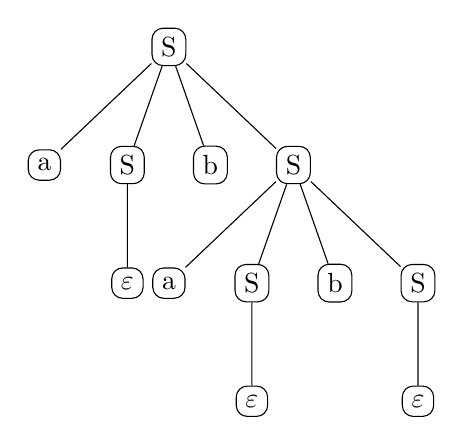
\begin{tikzpicture}[sibling distance=3em,
  every node/.style = {shape=rectangle, rounded corners,
    draw, align=center}]
  \node {S}
    child { node {a} }
    child { node {S}
      child { node {$\varepsilon$}}
    }
    child { node {b} }
    child { node {S}
      child {node {a}}
      child { node {S}
        child { node {$\varepsilon$}}
      }
      child { node {b} }
      child { node {S}
          child {node {$\varepsilon$}}
        }
      };
\end{tikzpicture}}
        \end{center}
        \caption{Дерева вывода цепочки $abab$ в грамматике~\ref{eq:grammar}}
        \label{fig:derivation_tree_example}
    \end{marginfigure}
    
\end{example}

\begin{theorem}
    Пусть $G = \langle \Sigma, N, P, S \rangle$~--- КС-грамматика.
    Вывод $S \derives \alpha$, где $\alpha \in (N \cup \Sigma)^*, \alpha \neq \varepsilon$ существует $\Leftrightarrow$ существует дерево вывода в грамматике $G$ с кроной $\alpha$.
\end{theorem}

\section{Пустота КС-языка}

\begin{theorem}
    Существует алгоритм, определяющий, является ли язык, порождаемый КС грамматикой, пустым.
\end{theorem}

\begin{proof}
    Следующая лемма утверждает, что если в КС языке есть выводимое слово, то существует другое выводимое слово с деревом вывода не глубже количества нетерминалов грамматики.
    Для доказательства теоремы достаточно привести алгоритм, последовательно строящий все деревья глубины не больше количества нетерминалов грамматики, и проверяющий, являются ли такие деревья деревьями вывода.
    Если в результате работы алгоритма не удалось построить ни одного дерева, то грамматика порождает пустой язык.
\end{proof}

\begin{lemma}
    Если в данной грамматике выводится некоторая цепочка, то существует цепочка, дерево вывода которой не содержит ветвей длиннее $m$, где $m$~--- количество нетерминалов грамматики.
\end{lemma}

\begin{proof}
    Рассмотрим дерево вывода цепочки $\omega$. Если в нем есть 2 узла, соответствующих одному нетерминалу A, обозначим их $n_1$ и $n_2$.

    Предположим, $n_1$ расположен ближе к корню дерева, чем $n_2$.

    Вывод цепочки $\omega$ имеет следующий вид:
    \[S \derives \alpha A_{n_1} \beta \derives \alpha \omega_1 \beta; S \derives \alpha \gamma A_{n_2} \delta \beta \derives \alpha \gamma \omega_2 \delta \beta \derives \omega,\]
    при этом $\omega_2$ является подцепочкой $\omega_1$.

    Заменим в изначальном дереве узел $n_1$ на $n_2$. Полученное дерево является деревом вывода цепочки $\alpha \omega_2 \delta$.

    Повторяем процесс замены одинаковых нетерминалов до тех пор, пока в дереве не останутся только уникальные нетерминалы.

    В полученном дереве не может быть ветвей длины большей, чем $m$.

    По построению оно является деревом вывода.
\end{proof}


\section{Нормальная форма Хомского}
\label{section:CNF}

\begin{definition}[Нормальная форма Хомского]
    Контекстно-свободная грамматика $\langle \Sigma, N, P, S\rangle$ находится в \emph{Нормальной Форме Хомского}, если она содержит только правила следующего вида:
    \begin{itemize}
        \item $A \to B C$, где $A, B, C \in N$, а стартовый нетерминал $S$ не содержится в правой части правила.
        \item $A \to a$, где $A \in N$, $a \in \Sigma$.
        \item $S \to \varepsilon$: только из стартового нетерминала выводима пустая строка.
    \end{itemize}
\end{definition}

\begin{theorem}
    Любую КС грамматику можно преобразовать в НФХ.
\end{theorem}

\begin{proof}
    Алгоритм преобразования в НФХ состоит из следующих шагов:
    \begin{itemize}
        \item Замена неодиночных терминалов
        \item Удаление длинных правил
        \item Удаление $\varepsilon$-правил
        \item Удаление цепных правил
        \item Удаление бесполезных нетерминалов
    \end{itemize}
    То, что каждый из этих шагов преобразует грамматику к эквивалентной, при этом является алгоритмом, доказано в следующих леммах.
\end{proof}

\begin{lemma}
    Для любой КС-грамматики можно построить эквивалентную, которая не содержит правила с неодиночными терминалами.
\end{lemma}

\begin{proof}
    Каждое правило $A \to B_0 B_1 \dots B_k$, $k \geq 1$ заменить на множество правил, где $C_i$~--- новый нетерминал:
    \begin{align*}
        A   & \to C_0 C_1 \dots C_k \\
        C_0 & \to B_0               \\
        C_1 & \to B_1               \\
            & \dots                 \\
        C_k & \to B_k
    \end{align*}
\end{proof}

\begin{lemma}
    Для любой КС-грамматики можно построить эквивалентную, которая не содержит правил длины больше 2.
\end{lemma}

\begin{proof}
    Каждое правило $A \to B_0 B_1 \dots B_k$, $k \geq 2$ заменить на множество правил:
    \begin{align*}
        A       & \to B_0 C_0         \\
        C_0     & \to B_1 C_1         \\
                & \dots               \\
        C_{k-3} & \to B_{k-2} C_{k-2} \\
        C_{k-2} & \to B_{k-1} B_k
    \end{align*}
\end{proof}


\begin{lemma}
    Для любой КС-грамматики можно построить эквивалентную, не содержащую $\varepsilon$-правил.
\end{lemma}

\begin{proof}
    Рекурсивно определим $\varepsilon$-правила:
    \begin{itemize}
        \item $A \to \varepsilon$~--- $\varepsilon$-правило
        \item $A \to B_0 \dots B_k$~--- $\varepsilon$-правило, если $\forall i$: $B_i$~--- $\varepsilon$-правило.
    \end{itemize}
    Каждое правило $A \to B_0 B_1 \dots B_k$ заменяем на множество правил, где каждое $\varepsilon$-правило удалено во всех возможных комбинациях.
\end{proof}

\begin{lemma}
    Для любой КС-грамматики можно построить эквивалентную, не содержащую цепные правила.
\end{lemma}

\begin{proof}
    \emph{Цепное правило}~--- правило вида $A \to B\text{, где } A, B \in N$.
    \emph{Цепная пара}~--- упорядоченная пара $(A,B)$, в которой $A\derives B$, используя только цепные правила.

    Алгоритм:
    \begin{enumerate}
        \item Найти все цепные пары в грамматике $G$.
              Найти все цепные пары можно по индукции:
              Базис: $(A,A)$~--- цепная пара для любого нетерминала, так как $A\derives A$ за ноль шагов.
              Индукция: Если пара $(A,B_0)$~--- цепная, и есть правило $B_0 \to B_1$, то $(A,B_1)$~--- цепная пара.
        \item Для каждой цепной пары $(A,B)$ добавить в грамматику $G'$ все правила вида $A \to a$, где $B \to a$~--- нецепное правило из $G$.
        \item Удалить все цепные правила
    \end{enumerate}
    Пусть $G$~--- контекстно-свободная грамматика. $G'$~--- грамматика, полученная в результате применения алгоритма к $G$. Тогда $L(G)=L(G')$.
\end{proof}

\begin{definition}[Порождающий и непорождающий нетерминалы]
    Нетерминал $A$ называется \emph{порождающим}, если из него может быть выведена конечная терминальная цепочка.
    Иначе он называется \emph{непорождающим}.
\end{definition}

\begin{lemma}
    Можно удалить все бесполезные (непорождающие) нетерминалы.
\end{lemma}

\begin{proof}
    После удаления из грамматики правил, содержащих непорождающие нетерминалы, язык не изменится, так как непорождающие нетерминалы по определению не могли участвовать в выводе какого-либо слова.

    Алгоритм нахождения порождающих нетерминалов:
    \begin{enumerate}
        \item Множество порождающих нетерминалов пустое.
        \item Найти правила, не содержащие нетерминалов в правых частях и добавить нетерминалы, встречающихся в левых частях таких правил, в множество.
        \item Если найдено такое правило, что все нетерминалы, стоящие в его правой части, уже входят в множество, то добавить в множество нетерминалы, стоящие в его левой части.
        \item Повторить предыдущий шаг, если множество порождающих нетерминалов изменилось.
    \end{enumerate}
    В результате получаем множество всех порождающих нетерминалов грамматики, а все нетерминалы, не попавшие в него, являются непорождающими.
    Их можно удалить.
\end{proof}

\begin{example}
    Приведем в Нормальную Форму Хомского однозначную грамматику правильных скобочных последовательностей: $S \to a S b S \mid \varepsilon$

    Первым шагом добавим новый нетерминал и сделаем его стартовым:
    \begin{align*}
        S_0 & \to S                        \\
        S   & \to a S b S \mid \varepsilon
    \end{align*}
    Заменим все терминалы на новые нетерминалы:
    \begin{align*}
        S_0 & \to S                        \\
        S   & \to L S R S \mid \varepsilon \\
        L   & \to a                        \\
        R   & \to b
    \end{align*}
    Избавимся от длинных правил:
    \begin{align*}
        S_0 & \to S                     \\
        S   & \to L S' \mid \varepsilon \\
        S'  & \to S S''                 \\
        S'' & \to R S                   \\
        L   & \to a                     \\
        R   & \to b
    \end{align*}
    Избавимся от $\varepsilon$-продукций:
    \begin{align*}
        S_0 & \to S \mid \varepsilon \\
        S   & \to L S'               \\
        S'  & \to S'' \mid S S''     \\
        S'' & \to R   \mid R S       \\
        L   & \to a                  \\
        R   & \to b
    \end{align*}
    Избавимся от цепных правил:
    \begin{align*}
        S_0 & \to L S' \mid \varepsilon \\
        S   & \to L S'                  \\
        S'  & \to b \mid R S \mid S S'' \\
        S'' & \to b \mid R S            \\
        L   & \to a                     \\
        R   & \to b
    \end{align*}
\end{example}

\begin{definition}[Ослабленная нормальная форма Хомского (ОНФХ)]
    \label{defn:wCNF}
    Контекстно-свободная грамматика $\langle \Sigma, N, P, S\rangle$ находится в \emph{ослабленной Нормальной Форме Хомского}, если она содержит только правила следующего вида:
    \begin{itemize}
        \item $A \to B C$, где $A, B, C \in N$;
        \item $A \to a$, где $A \in N$, $a \in \Sigma$;
        \item $A \to \varepsilon$, где $A \in N$.
    \end{itemize}
\end{definition}

То есть ослабленная НФХ отличается от НФХ тем, что:
\begin{enumerate}
    \item $\varepsilon$ может выводиться из любого нетерминала;
    \item $S$ может появляться в правых частях правил.
\end{enumerate}


\section{Лемма о накачке}

\begin{lemma}
    Пусть $L$~--- контекстно-свободный язык над алфавитом $\Sigma$, тогда существует такое $n$, что для любого слова $\omega \in L$, $|\omega| \geq n$ найдутся слова $u,v,x,y,z\in \Sigma^*$, для которых верно: $uvxyz = \omega, vy\neq \varepsilon,|vxy|\leq n$ и для любого $k \geq 0$  $uv^kxy^kz \in L$.
\end{lemma}

\begin{proofSketch}

    \begin{enumerate}
        \item Для любого КС языка можно найти грамматику в нормальной форме Хомского.
        \item Очевидно, что если брать достаточно длинные цепочки, то в дереве вывода этих цепочек, на пути от корня к какому-то листу обязательно будет нетерминал, встречающийся минимум два раза. Если $m$~--- количество нетерминалов в НФХ, то длины $2^{m+1}$ должно хватить. Это и будет $n$ из леммы.
        \item Возьмём путь, на котором есть хотя бы дважды повторяется некоторый нетерминал. Скажем, это нетерминал  $N_1$. Пойдём от листа по этому пути. Найдём первое появление $N_1$. Цепочка, задаваемая поддеревом для этого узла~--- это $x$ из леммы.
        \item Пойдём дальше и найдём второе появление $N_1$. Цепочка, задаваемая поддеревом для этого узла~--- это $vxy$ из леммы.
        \item Теперь мы можем копировать кусок дерева между этими повторениями $N_1$ и таким образом накачивать исходную цепочку.
    \end{enumerate}
    Надо только проверить выполнение ограничений на длины.
    Нахождение разбиения и пример накачки продемонстрированы на рисунках~\ref{fig:pumping1} и~\ref{fig:pumping2}.
\end{proofSketch}

\begin{marginfigure}
    \centering
    \input{figures/cfl/pumping1.tex}
    \caption{Разбиение цепочки для леммы о накачке}
    \label{fig:pumping1}
\end{marginfigure}

\begin{marginfigure}
    \begin{center}
    \begin{subfigure}{\marginparwidth}
        \centering
        \input{figures/cfl/pumping0.tex}
        \caption{$k = 0$.}
        % \label{fig:f1}
    \end{subfigure}
    
    \begin{subfigure}{\linewidth}
        \centering
        \input{figures/cfl/pumping2.tex}
        \caption{$k = 2$.}
        % \label{fig:f2}
    \end{subfigure}
\end{center}
    \caption{Пример накачки цепочки с рисунка~\ref{fig:pumping1}}
    \label{fig:pumping2}
\end{marginfigure}

Для примера предлагается проверить неконтекстно-свободность языка $L=\{a^nb^nc^n \mid n>0\}$.

\section{Замкнутость КС языков относительно операций}

\begin{theorem}
    Контекстно-свободные языки замкнуты относительно следующих операций:
    \begin{enumerate}
        \item Объединение: если $L_1$ и $L_2$~--- контекстно-свободные языки, то и $L_3 = L_1 \cup L_2$~--- контекстно-свободный.
        \item Конкатенация: если $L_1$ и $L_2$~--- контекстно-свободные языки, то и $L_3 = L_1 \cdot L_2$~--- контекстно-свободный.
        \item Замыкание Клини: если $L_1$~--- контекстно-свободный, то и $L_2 = \bigcup\limits_{i=0}^{\infty} L_1^i $~--- контекстно-свободный.
        \item Разворот: если $L_1$~--- контекстно-свободный, то и $L_2 = {L_1}^r = \{ l^r \mid l \in L_1\}$ является контекстно-свободным.
        \item Пересечение с регулярными языками: если $L_1$~--- контекстно-свободный, а $L_2$~--- регулярный, то  $L_3 = L_1 \cap L_2$~--- контекстно-свободный.
        \item Разность с регулярными языками: если $L_1$~--- контекстно-свободный, а $L_2$~--- регулярный, то  $L_3 = L_1 \setminus L_2$~--- контекстно-свободный.
    \end{enumerate}
\end{theorem}
\begin{proof}
    Для доказательства пунктов 1--4 можно построить КС грамматику нового языка имея грамматики для исходных.
    Будем предполагать, что множества нетерминальных символов различных грамматик для исходных языков не пересекаются.
    \begin{enumerate}
        \item $G_1=\langle\Sigma_1,N_1,P_1,S_1\rangle$~--- грамматика для $L_1$, $G_1=\langle\Sigma_2,N_2,P_2,S_2\rangle$~--- грамматика для $L_2$, тогда 
        \[G_3=\langle\Sigma_1 \cup \Sigma_2, N_1 \cup N_2 \cup \{S_3\}, P_1 \cup P_2 \cup \{S_3 \to S_1 \mid S_2\} ,S_3\rangle\] ---~грамматика для $L_3$.
        \item $G_1=\langle\Sigma_1,N_1,P_1,S_1\rangle$~--- грамматика для $L_1$, $G_1=\langle\Sigma_2,N_2,P_2,S_2\rangle$~--- грамматика для $L_2$, тогда $G_3=\langle\Sigma_1 \cup \Sigma_2, N_1 \cup N_2 \cup \{S_3\}, P_1 \cup P_2 \cup \{S_3 \to S_1 S_2\} ,S_3\rangle$~--- грамматика для $L_3$.
        \item $G_1=\langle\Sigma_1,N_1,P_1,S_1\rangle$~--- грамматика для $L_1$, тогда $G_2=\langle\Sigma_1, N_1 \cup \{S_2\}, P_1 \cup \{S_2 \to S_1 S_2\ \mid \varepsilon\}, S_2\rangle$~--- грамматика для $L_2$.
        \item $G_1=\langle\Sigma_1,N_1,P_1,S_1\rangle$~--- грамматика для $L_1$, тогда $G_2=\langle\Sigma_1, N_1, \{N^i \to \omega^R \mid N^i \to \omega \in P_1 \}, S_1\rangle$~--- грамматика для $L_2$.
    \end{enumerate}

    Чтобы доказать замкнутость относительно пересечения с регулярными языками, построим по КС грамматике рекурсивный автомат $R_1$, по регулярному выражению~--- детерминированный конечный автомат $R_2$, и построим их прямое произведение $R_3$.
    Переходы по терминальным символам в новом автомате возможны тогда и только тогда, когда они возможны одновременно и в исходном рекурсивном автомате и в исходном конечном.
    За рекурсивные вызовы отвечает исходный рекурсивный автомат.
    \marginnote{TODO: Вот тут RSM очень внезапно вылез}
    Значит цепочка принимается $R_3$ тогда и только тогда, когда она принимается одновременно $R_1$ и $R_2$: так как состояния $R_3$~--- это пары из состояния $R_1$ и $R_2$, то по трассе вычислений $R_3$ мы всегда можем построить трассу для $R_1$ и $R_2$ и наоборот.

    Чтобы доказать замкнутость относительно разности с регулярным языком, достаточно вспомнить, что регулярные языки замкнуты относительно дополнения, и выразить разность через пересечение с дополнением:
    \[L_1 \setminus L_2 = L_1 \cap \overline{L_2} \qedhere\]
\end{proof}

\begin{theorem}
    Контекстно-свободные языки не замкнуты относительно следующих операций:
    \begin{enumerate}
        \item Пересечение: если $L_1$ и $L_2$~--- контекстно-свободные языки, то и $L_3 = L_1 \cap L_2$~--- не контекстно-свободный.
        \item Разность: если $L_1$ и $L_2$~--- контекстно-свободные языки, то и $L_3 = L_1 \setminus L_2$~--- не контекстно-свободный.
    \end{enumerate}
\end{theorem}

\begin{proof}
    Чтобы доказать незамкнутость относительно пресечения, рассмотрим языки $L_1 = \{a^n b^n c^k \mid n \geq 0, k \geq 0\}$ и $L_2 = \{a^k b^n c^n \mid n \geq 0, k \geq 0\}$.
    Очевидно, что $L_1$ и $L_2$~--- контекстно-свободные языки.
    Рассмотрим $L_3 = L_1 \cap L_2 = \{a^n b^n c^n \mid n \geq 0\}$.
    $L_3$ не является контекстно-свободным по лемме о накачке для контекстно-свободных языков.

    Чтобы доказать незамкнутость относительно разности проделаем следующее.
    \begin{enumerate}
        \item Рассмотрим языки $L_4 = \{a^m b^n c^k \mid m \neq n, k \geq 0\}$ и $L_5 = \{a^m b^n c^k \mid n \neq k, m \geq 0\}$.
              Эти языки являются контекстно-свободными.
              Это легко заметить, если знать, что язык $L'_4 = \{a^m b^n c^k \mid 0 \leq m < n, k \geq 0\}$ задаётся следующей грамматикой:
              \begin{align*}
                  S & \to S c & T & \to a T b \\
                  S & \to T   & T & \to T b   \\
                    &         & T & \to b.
              \end{align*}
        \item Рассмотрим язык $L_6 = \overline{L'_6} = \overline{\{a^n b^m c^k \mid n \geq 0, m \geq 0, k \geq 0\}}$.
              Данный язык является регулярным\sidenote{Предлагаем читателю самостоятельно написать регулярное выражение, задающее этот язык.}.
        \item Рассмотрим язык $L_7 = L_4 \cup L_5 \cup L_6$~--- контекстно-свободный, так как является объединением контекстно-свободных.
        \item Рассмотрим $\overline{L_7} = \{a^n b^n c^n \mid n \geq 0\} = L_3$: $L_4$ и $L_5$ задают языки с правильным порядком символов, но неравным их количеством, $L_6$ задаёт язык с неправильным порядком символов.
              Из предыдущего пункта мы знаем, что $L_3$  не является контекстно-свободным.
              \qedhere
    \end{enumerate}
\end{proof}




%\section{Вопросы и задачи}
%\begin{enumerate}
%  \item Постройте дерево вывода цепочки $w=aababb$ в грамматике $G=\langle\{a,b\},\{S\},\{S\rightarrow \varepsilon \ | \ a \ S \ b \ S \}, S \rangle$.
%  \item Постройте все левосторонние выводы цепочки $w=ababab$ в грамматике $G=\langle\{a,b\},\{S\},\{S\rightarrow \varepsilon \ | \ a \ S \ b \ | S \ S\}, S \rangle$.
%  \item Постройте все правосторонние выводы цепочки $w=ababab$ в грамматике $G=\langle\{a,b\},\{S\},\{S\rightarrow \varepsilon \ | \ a \ S \ b \ | S \ S\}, S \rangle$.
%  \item \label{t1}Постройте все деревья вывода цепочки $w=ababab$ в грамматике $G=\langle\{a,b\},\{S\},\{S\rightarrow \varepsilon \ | \ a \ S \ b \ | S \ S\}, S \rangle$, соответствующие левосторонним выводам.
%  \item \label{t2}Постройте все деревья вывода цепочки $w=ababab$ в грамматике $G=\langle\{a,b\},\{S\},\{S\rightarrow \varepsilon \ | \ a \ S \ b \ | S \ S\}, S \rangle$, соответствующие правосторонним выводам.
%\end{enumerate}
